\problemname{Correcting Cheeseburgers}

Cheeseburgers are serious business. They are the most delicious food on earth, but there is a lot of room for error when making a cheeseburger.
Even otherwise capable cooks often mess up the order of the assembled ingredients.

The only correct order of ingredients between the buns is, \emph{of course}, as following from top to bottom:
\begin{enumerate}
  \item Ketchup \& Mustard
  \item Beef Tomato
  \item Pickles
  \item Red Onions
  \item Cheddar Cheese
  \item Garlic
  \item Salt \& Pepper
  \item Beef Patty, medium grilled
  \item Corn Salad
  \item Mayonnaise
\end{enumerate}
Any deviation from this order is completely unacceptable. Therefore it is sometimes necessary to reassemble a cheeseburger.

Space on an average plate and social norms are rather restrictive when it comes to operating on a cheeseburger.
The only feasible operation is the bit-shuffle (burger-ineptly-transformed).
The bit-shuffle separates the entire burger into four parts of contiguous ingredients $a$, $b$, $c$ and $d$ and arranges them in the new order $c\ a\ d\ b$.
The size of each of the four parts is selectable and may be zero.

Since the burger cools rapidly we are interested in the minimum required bit-shuffles to arrive at an acceptable burger.

Each given cheeseburger consists of $n$ unique ingredients labeled from 1 to $n$. The correct order is always
the natural order $1\ 2 \dots n$.


\begin{figure}[!h]
	\centering
	\subfigure{	
		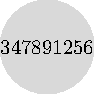
\includegraphics[scale=1]{fig_0_0.pdf}
	}
	\qquad
	\subfigure{	
		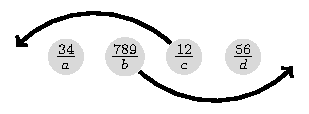
\includegraphics[scale=1]{fig_0_1.pdf}
	}
	\qquad
	\subfigure{	
		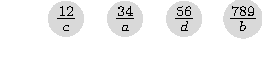
\includegraphics[scale=1]{fig_0_2.pdf}	
	}
	\caption{Illustration of the first sample input.}
\end{figure}

\begin{figure}[!h]
	\centering
	\subfigure{	
		
\includegraphics[scale=1]{fig_1_0.pdf}
	}
	\qquad
	\subfigure{	
		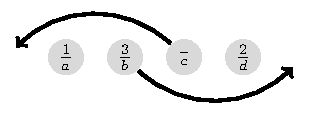
\includegraphics[scale=1]{fig_1_1.pdf}
	}
	\qquad
	\subfigure{	
		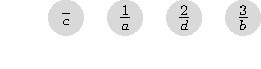
\includegraphics[scale=1]{fig_1_2.pdf}
	}
	\caption{Illustration of the second sample input.}
\end{figure}


\section*{Input}

The input consists of:
\begin{itemize}
\item one line with an integer $n$ ($1 \leq n \leq 10$), where $n$ is the number of ingredients used;
\item one line with $n$ integers describing the order of the ingredients of the given cheeseburger. The ingredients are numbered from $1$ to $n$.
\end{itemize}

\section*{Output}

Output the minimum number of bit-shuffles to correct the given cheeseburger. 
